\documentclass{article}
\usepackage[school,simplified]{pgf-umlcd}
\usetikzlibrary{calc}
\usetikzlibrary{positioning}
\usepackage{fullpage}
\usepackage{fancyhdr}
\pagestyle{fancy}
\lhead{}
\rhead{}
\chead{}
\rfoot{\thepage}
\lfoot{Martin Baumgaertner - Tous droits résérvés (- : privé, + : public)\\ 
(Flèche vide/flèche = Héritage = être, Flèche pleine/Losange = Aggrégation = avoir)}
\cfoot{}
\renewcommand{\headrulewidth}{0pt}
\begin{document}  

 
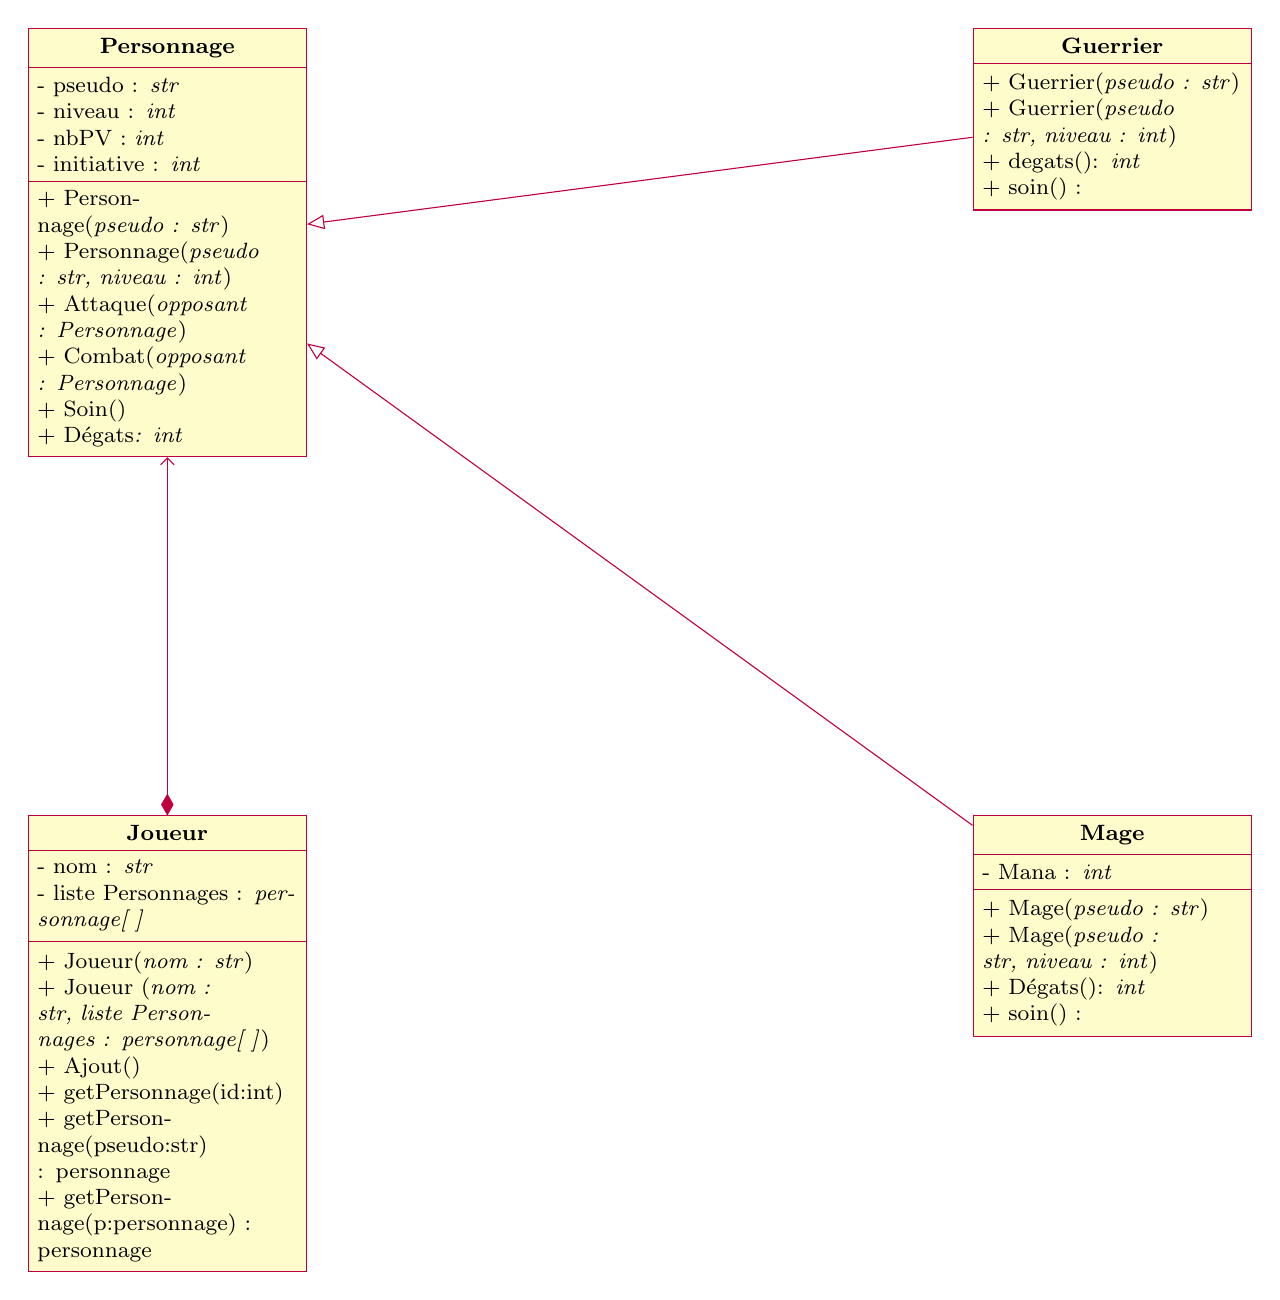
\begin{tikzpicture}[font=\footnotesize] 



\begin{class}[text width = 3.3cm, yshift=-5mm]{Personnage}{0,10}
    \attribute{- pseudo : \textit{str}}
    \attribute{- niveau : \textit{int}}
    \attribute{- nbPV : \textit{int}}
    \attribute{- initiative : \textit{int}}
    \operation{+ Personnage(\textit{pseudo : str})}
    \operation{+ Personnage(\textit{pseudo : str, niveau : int})}
    \operation{+ Attaque(\textit{opposant : Personnage})}
    \operation{+ Combat(\textit{opposant : Personnage})}
    \operation{+ Soin()}
    \operation{+ Dégats\textit{: int}}


\end{class}

\begin{class}[text width = 3.3cm, yshift=-5mm]{Joueur}{0,0}
    \attribute{- nom : \textit{str}}
    \attribute{- liste Personnages : \textit{personnage[ ]}}
    \operation{+ Joueur(\textit{nom : str})}
    \operation{+ Joueur (\textit{nom : str, liste Personnages : personnage[ ]})}
    \operation{+ Ajout()}
    \operation{+ getPersonnage(id:int)}
    \operation{+ getPersonnage(pseudo:str) : personnage}
    \operation{+ getPersonnage(p:personnage) : personnage}
\end{class}


\begin{class}[text width = 3.3cm, yshift=-5mm]{Guerrier}{12,10}
    \inherit{Personnage}
    \operation{+ Guerrier(\textit{pseudo : str})}
    \operation{+ Guerrier(\textit{pseudo : str, niveau : int})}
    \operation{+ degats(): \textit{int}}
    \operation{+ soin() :}
\end{class}

\begin{class}[text width = 3.3cm, yshift=-5mm]{Mage}{12,0}
    \inherit{Personnage}
    \attribute{- Mana : \textit{int}}
    \operation{+ Mage(\textit{pseudo : str})}
    \operation{+ Mage(\textit{pseudo : str, niveau : int})}
    \operation{+ Dégats(): \textit{int}}
    \operation{+ soin() :}
\end{class}

\composition{Joueur}{}{}{Personnage}

\end{tikzpicture}
\end{document}